\section{Variational Message Passing}

Let $\Theta$ be the set of hidden variables and $X$ be the observed variables.
parametric family of distributions. We use capital letters $P$, $Q$ to
represent distributions, and corresponding small letters $p$, $q$ to denote
its probabilistic density function or probability mass function.
Variational inference approximates the posterior distribution
$P_{\Theta|X}$ with a distrbution $Q_{\Theta}$ from a
A simple choice of the
approximating
family is,
\begin{equation*}
	q(\Theta) = \prod_{\theta \in \Theta} q(\theta)
\end{equation*}
, the fully factorized family over the parameters. This choice assumes that
all hidden variables are independent in the approximate distribution. Since
the independence assumption may not be true in the posterior distribution, the
algorithm may not be able to find the exact posterior distribution. The
algorithm iteratively minimizes the Kullback-Leibler divergence
$\mathrm{KL}(Q||P)$ between the approximate distribution and
the true distribution so that the approximate distribution is as close as
possible to the true posterior. Although the KL divergence cannot be computed
without knowing the true posterior, it is not necessary to
directly optimize the KL divergence. Instead, the algorithm maxmizes the
evidence lower bound (ELBO) 
\begin{equation}
	\label{eqn:ELBO}
	\mathcal{L}(Q) = E_Q[\ln p(\Theta, X) - \ln q(\Theta)] 
\end{equation} 
, maximizing which is equivalent to minimizing the KL divergence. ELBO only
involves the expectation of the log likelihoods in terms of the approximate
distribution $Q$ and it is straight forward to calculate. 

Separating out terms related to one of the hidden variables $\theta \in
\Theta$ and let $F_{(\cdot)}$ be the parent of the variable and
$\mathrm{C}_{(\cdot)}$ be the set of children of the variable, the ELBO can be
rewritten as
\begin{align*}
	&\mathcal{L}(Q) = -\mathrm{KL}(Q_\theta || \tilde{P}_\theta) +
	\mathrm{Const}(\theta) \numberthis \label{eqn:ELBO_one_term}
\end{align*}
, where $\mathrm{Const}(\theta)$ is a constant with respect to $\theta$ and $\tilde{P_\theta}$ is defined as
\begin{align*}
	&\ln\tilde{p}(\theta) = E_{Q_{\Theta \backslash
	\theta}}[\ln p(\theta|\mathrm{F}_\theta) + \sum_{\phi \in
	\mathrm{C}_\theta }p(\phi|\mathrm{F}_\phi)] + Z
\end{align*}
$Z$ is a normalizing constant. The KL divergence is always non-negative. It
equals to zero if and only if the two distributions are the same. Therefore,
setting $Q_\theta$ to $\tilde{P}_\theta$ maximizes the ELBO with regard to
$\theta$.  Since the model is in exponential family and have conjugate priors,
all terms in $\ln \tilde{p}(\theta)$ has the same form of the dot product of
parameters and sufficient statistics except the normalizing constant.
Therefore, the ELBO is maximized by letting $\ln q(\theta)$ have the same form
as $p(\theta|\mathrm{F}_\theta)$ and setting the parameters to those of
$\tilde{P_\theta}$.  In the coin flipping case, if the probability of head has
$\mathrm{Beta}(\alpha, \beta)$ prior,
\begin{align*}
\ln\tilde{p}(\phi) &= [\alpha - 1 \quad \beta - 1] 
	\begin{bmatrix} \ln \phi \\ \ln(1-\phi) \end{bmatrix}  \\
	&+ [H \quad N-H]  \begin{bmatrix} \ln \phi \\ \ln(1-\phi) \end{bmatrix} + Z
\end{align*}
The ELBO is maximized when the $Q$ is set to $\mathrm{Beta}(\alpha + H,
\beta + N - H)$. Note in the one coin model, $Q$ is exactly the true
posterior in \eqnref{eqn:coin_posterior} because the independence assumption
naturally holds for a univariate distribution.

\begin{figure}[h]
	\includegraphics[scale=0.5]{figs/two_coins_latent.eps}
	\label{fig:two_coins_latent}
	\caption{Introducing additional hidden variables to mixture model}
\end{figure}

Mixture models (e.g. flipping two coins) are no longer in Exponential conjugate
family. To apply the variational algorithm, the trick is to introduce
additional hidden variables. For example, we can add the choice of the coins
(i.e. $z_i$ in \figref{fig:two_coins_latent}) for each of the outcomes. Let
$z_{ik} = 1$ if $z_i = k$, $z_{ik} = 0$ otherwise, and $x_{i} = 1$ if $x_i$ is
head, $x_{i} = 0$ if $x_i$ is tail, the log likelihood of
$x_i$ is 
\begin{align*}
	\ln p(x_i|\phi_1, \phi_2, z_i) = \sum_{k=1}^2 z_{ik} [x_{i} \quad 1-x_{i}]
\begin{bmatrix} \ln \phi_k \\ \ln (1-\phi_k) \end{bmatrix}
\end{align*}
The log likehood has the same forms as the prior $\ln f(\phi_k; \alpha, \beta)$.
Hence the model is conjugate.

The updates to the parameters of approximate distributions $Q$
are the aggregation of terms that either only depends on the parent or depends
on one child and the other parents of it. The terms in the updates can be
computed locally at the neighbours of the updated random variable.  For
example, the update of $z_i$'s parameters in the
two coins model is
\begin{equation}
	E[\ln \pi] + E[\ln p(x|\phi)]
\end{equation}
The first term can be computed locally at $\pi$ and the second term can be
computed locally at $x_i$ given $\phi_1$ and $\phi_2$.  The VMP algorithm
defines the terms as messages to be sent along both directions of edges in the
Bayesian network. In each step, one of the vertecies is chosen to pull
messages from its neighbours and update itself by aggregating the messages.
If a message is from the child and also depends on co-parents, the child will
pull messages from the co-parent as well. 
